To begin rendering a scene, we must first establish our viewpoint, often represented by a virtual camera. We can define the camera using the following parameters: 
$$\Vec{P} \text{ is a three dimensional vector representing the camera's position}$$
$$\hat{V} \text{ is a \textbf{normalized} three dimensional vector representing the camera's direction}$$
$$ w \text{ is the viewport width} $$
$$ h \text{ is the viewport height} $$
$$ z \text{ is the distance of the viewport's near plane from the position along $\hat{V}$}$$

\begin{tcolorbox}
   \textbf{Note:} all three dimensional vectors relating to position or direction will be in the form $\begin{bmatrix} x \\ y \\ z \end{bmatrix}$ unless otherwise specified.
\end{tcolorbox}

\begin{figure}[h]
    \centering
    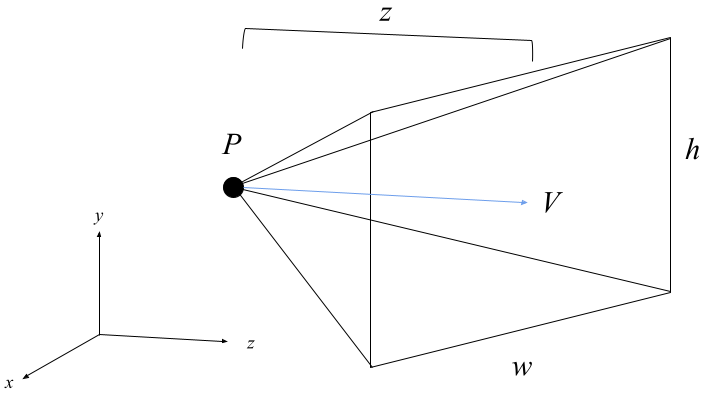
\includegraphics[scale=0.4]{figures/CameraDefinition.png}
    \caption{Visualization of the camera definition}
    \label{fig:camera_def}
\end{figure}